\documentclass{siproblemset}

% See Command Reference.tex/pdf for the full command reference

% SI Session Information
\course{MTH 1321}       % the course of your SI
\sessionnum{9}          % (optional) specify the session number
\sessiondate{10/2/19}   % the date of the session

% Topics Covered Box (optional)
\warmup{Topics Covered Box}
\topic{Use this section}
\topic{for listing the topics}
\topic{covered in this SI}
\cooldown{(this box is optional, delete the code to get rid of it)}

% Worksheet Information
\title{Template\linebreak and Instructions}   % title of worksheet
\sections{Sections X.Y and A.B}               % (optional) book chapters/sections
\withnamespace                                % (optional) adds the 'Name: ____' section

\begin{document}
    % Make the title, session info header, topics covered box, and name space
    \maketitle
    
    %% First Activity
    % use \activity to mark the start of a new activity section (restarts numbering)
    \activity{Type of Activity}{Name of Activity}{Instructions}{time allotted}
    
    Using plain text in an activity is perfectly fine! In fact, you can use plain text in most places. Here is a worked example of an activity title:
    \smallsp
    
    %% Warmup
    \activity{Warmup}{Basic Question Types}{Work with a \textbf{partner} to answer these questions. Try not to use your notes.}{15 minutes}
    
    % Free Response Questions
    \frq{To make a Free Response Question, use the \cs{frq[qnum]\{question text\}} command.}
    \tinysp
    \frq[1234]{All questions automatically number themselves. To manually change the number of a single question, specify the number in the optional argument. Due to package limitations, however, the number will always be incremented.}
    \tinysp
    \changequestionnumber{200}
    \frq{Using \cs{changequestionnumber}, it is also possible to advance the question numbers of all following questions.}
    \tinysp
    
    % True/False Questions
    \tfq{True/False questions are very easy to create as well! \cs{tfq[qnum]\{question text\}} does the trick and can be individually numbered just like FRQs can.}
    \newpage
    
    
    %% Advanced Question Making
    \activity{Activity 1}{Advance Question Creation}{There are two types of advanced questions, multiple-choice questions and multi-part questions.}{30 minutes}
    
    % Multiple-choice questions
    \mcq{Multiple-choice questions are made using the \cs{mcq[cols][qnum]\{question text\}\{choices\}} command. Notice the arguments that this command takes:}{
        \task \texttt{cols}: number of choice columns (default: 1)
        \task \texttt{qnum}: number of the question (see above) (default: current question number)
        \task \texttt{question text}: the text of the question
        \task \texttt{choices}: the list of choices. Each choice is prefaced with the macro \cs{task} and on its own line.
        \tinysp
        \task Note also that there \textit{can} be space between choices.
    }
    \tinysp
    \mcq[3]{The \texttt{cols} argument is perhaps the most powerful feature of this command. It specifies the amount of columns of choices. Here is an example with \texttt{cols} set to \texttt{3}:}{
        \task Choice A
        \task Choice B
        \task Choice C
        \task*(2) Use \cs{task*(num)} to span multiple columns
        \task Choice D
        \task Choice E
        \task* Or just use \cs{task*} to span the remaining columns
        \task Choice F
        \task! Or use \cs{task!} to span \textit{all} of the columns.
    }
    \tinysp
    
    % Multi-part questions
    \begin{multipartquestion}
        The other type of advance question is the multi-part question. This type of question gives you complete flexibility with your question. A multi-part question is an environment \linebreak(\cs{begin\{multipartquestion\}}) which renumbers every question inside of it with letters, allowing you to do all kinds of things.
        \frq{You can add free-response questions,}
        \tinysp
        \tfq{true/false questions,}
        \newpage
        \mcq{and even multiple-choice questions!}{
            \task However, you \textit{cannot} place a multi-part question inside of another one.
        }
        \tinysp
        Here are a few examples of the things that you can do with such questions:
    \end{multipartquestion}
    
    % Multi-part question examples
    \begin{multipartquestion}
        What are the units of the derivative of the following functions?
        \frq{$s(t)$, $v(t)$, $a(t)$; $v(t)$ is the first derivative of $s(t)$, $a(t)$ is the first derivative of $v(t)$, $s(t)$ is in \SI{}{\centi\meter}, and $t$ is in \SI{}{\micro\second}.}
        \Smallsp
        \frq{$C(n)$; $C(n)$ gives the cost, in dollars, of $n$ widgets from the widget factory.}
        \tinysp
        \frq{$f(x)=x^2$; $x$ is in meters.}
        \tinysp
    \end{multipartquestion}
    Or something more advanced:
    \begin{multipartquestion}
        Given the graph below:
        
        \mbox{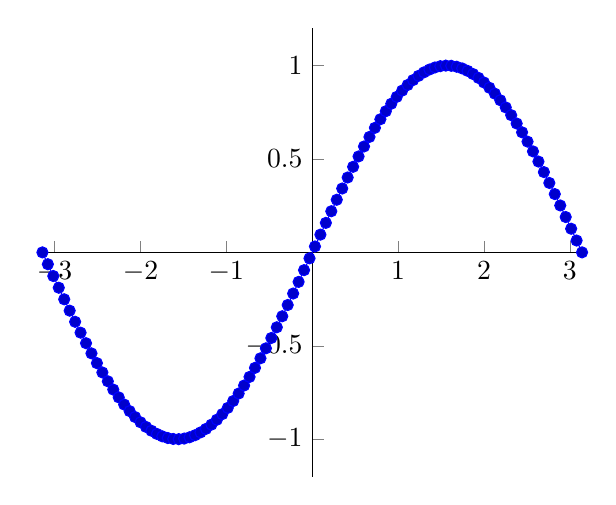
\begin{tikzpicture}[baseline=(current bounding box.north)]
            \begin{axis}[
            xmin=-pi,
            xmax=pi,
            ymin=-1.2,
            ymax=1.2,
            axis x line*=middle,
            axis y line*=middle,
            ]
            \addplot+[domain=-pi:pi, samples=100] {sin(deg(x))};
            \end{axis}
            \end{tikzpicture}}
        \parbox[t]{3.25in}{\vskip0pt
            \frq{What is the function $f(x)$?}
            \tinysp
            \frq{What is $f'(x)$?}
            \tinysp
            \frq{What is $f''(x)$?}
        }
    \end{multipartquestion}
    \newpage
    \begin{multipartquestion}
        Find the value of the following limits. If the limit does not exist, find the values of the left-hand and right-hand limits.
        \begin{multicols}{2}
            \frq{$\lim\limits_{x\rightarrow-2}f(x)$ and $\lim\limits_{x\rightarrow2}f(x)$}
            \mbox{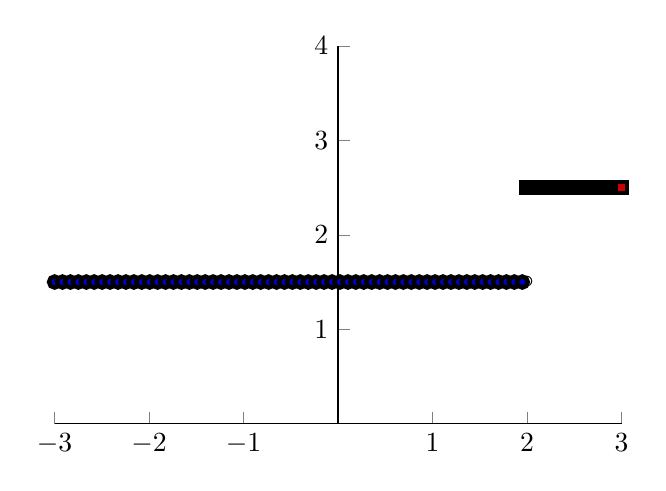
\begin{tikzpicture}[baseline=(current bounding box.north)]
                \begin{axis}[
                x=1.2cm,
                y=1.2cm,
                xmin=-3,
                xmax=3,
                ymin=0,
                ymax=4,
                axis x line*=middle,
                axis y line*=middle,
                every axis plot/.append style={ultra thick},
                samples=60
                ]
                \addplot+[black, domain=-3:1.95] {1.5};
                \addplot+[black, domain=2:3] {2.5};
                \node at (2,1.5) {$\circ$};
                \node at (2,2.5) {\textbullet};
                \end{axis}
                \end{tikzpicture}}
            \tinysp
            
            \frq{$\lim\limits_{x\rightarrow-2}f(x)$ and $\lim\limits_{x\rightarrow1}f(x)$}
            \mbox{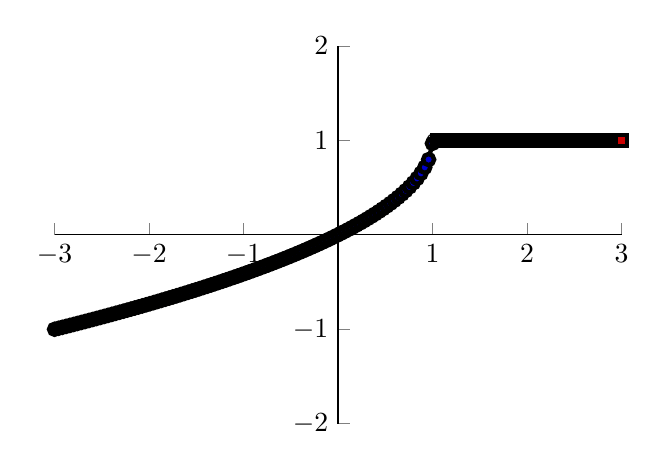
\begin{tikzpicture}[baseline=(current bounding box.north)]
                \begin{axis}[
                x=1.2cm,
                y=1.2cm,
                xmin=-3,
                xmax=3,
                ymin=-2,
                ymax=2,
                axis x line*=middle,
                axis y line*=middle,
                every axis plot/.append style={ultra thick},
                samples=100
                ]
                \addplot+[black, domain=-3:0.999] {1-sqrt(-x+1)};
                \addplot+[black, domain=1.05:3] {1};
                \node at (1,1) {$\circ$};
                \end{axis}
                \end{tikzpicture}}
            \tinysp
            
            \frq{$\lim\limits_{x\rightarrow-1}f(x)$ and $\lim\limits_{x\rightarrow0}f(x)$}
            \mbox{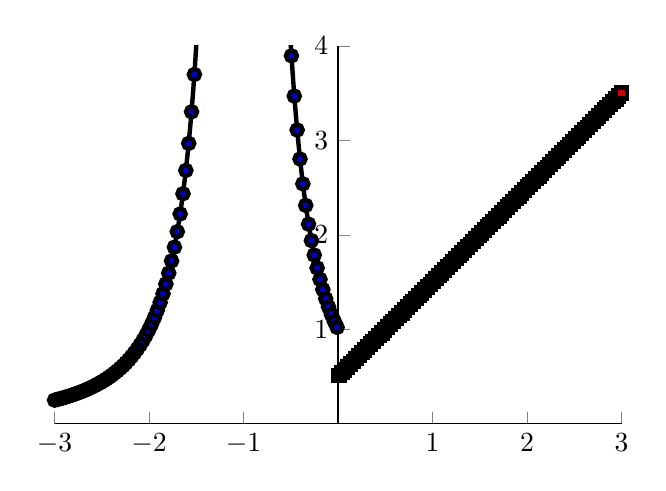
\begin{tikzpicture}[baseline=(current bounding box.north)]
                \begin{axis}[
                x=1.2cm,
                y=1.2cm,
                xmin=-3,
                xmax=3,
                ymin=0,
                ymax=4,
                axis x line*=middle,
                axis y line*=middle,
                every axis plot/.append style={ultra thick},
                samples=100
                ]
                \addplot+[black, domain=-3:-0.01,restrict y to domain =-20:100] {1/(x+1)^2};
                \addplot+[black, domain=0.01:3] {x+1/2};
                \node at (0,1) {$\circ$};
                \node at (0,0.5) {\textbullet};
                \end{axis}
                \end{tikzpicture}}
            \tinysp
            
            \frq{$\lim\limits_{x\rightarrow0}f(x)$ and $\lim\limits_{x\rightarrow2.5}f(x)$}
            \mbox{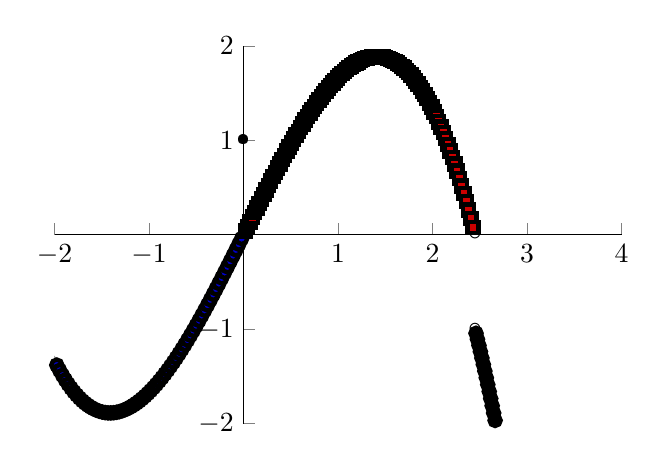
\begin{tikzpicture}[baseline=(current bounding box.north)]
                \begin{axis}[
                x=1.2cm,
                y=1.2cm,
                xmin=-2,
                xmax=4,
                ymin=-2,
                ymax=2,
                axis x line*=middle,
                axis y line*=middle,
                every axis plot/.append style={ultra thick},
                samples=100
                ]
                \addplot+[black, domain=-3:-0.02,restrict y to domain =-20:100] {-x^3/3+2*x};
                \addplot+[black, domain=0.02:2.43,restrict y to domain =-20:100] {-x^3/3+2*x};
                \addplot+[black, domain=2.46:4,restrict y to domain =-20:100] {-x^3/3+2*x-1};
                \node at (0,0) {$\circ$};
                \node at (0,1) {\textbullet};
                \node at (2.45,0) {$\circ$};
                \node at (2.45,-1) {$\circ$};
                \end{axis}
                \end{tikzpicture}}
            \tinysp
        \end{multicols}
        \tinysp
    \end{multipartquestion}

    % Multi-part multiple-choice question example
    \mcq[2]{Sometimes, you may want to make two columns of questions. In this case, a simple \cs{mcq[cols]} with spaces can same you some time over using a multi-part question:}{
        \task What is the meaning of life?
        \tinysp
        \task Which came first, the chicken or the egg?
        \tinysp
        \task Knock. Knock. Who's there?
        \tinysp
        \task Are we there yet?
        \tinysp
    }
    
    %% Spaces
    \activity{Activity 2}{Exploring Spaces}{Here is a list of the different space types. Of course, use \cs{vspace} and \cs{newpage}/\cs{pagebreak} for more fine-tuned control}{30 minutes}
    
    \frq{\cs{tinysp} $\cmp{1}$}
    \tinysp
    \frq{\cs{Tinysp} $\cmp{2}$}
    \Tinysp
    \frq{\cs{smallsp} $\cmp{3}$}
    \smallsp
    \frq{\cs{Smallsp} $\cmp{4}$}
    \Smallsp
    \frq{\cs{normalsp} $\cmp{5}$}
    \normalsp
    (continued on next page)
    \frq{\cs{Normalsp} $\cmp{6}$}
    \Normalsp
    \frq{\cs{largesp} $\cmp{7}$}
    \largesp
    (continued on next page)
    \newpage
    \frq{\cs{Largesp} $\cmp{8}$}
    \Largesp
    \frq{\cs{hugesp} $\cmp{9}$}
    \hugesp
    (continued on next page)
    \newpage
    \frq{\cs{Hugesp} $\cmp{10}$}
    \Hugesp
    
    \activity{Cooldown}{Math!}{Attempt to do these problems \textbf{alone} then discuss your answers with the people around you.}{15 minutes}
    
    Math is not only allowed, but it is encouraged! Just use \texttt{\$...\$} and \texttt{\$\$...\$\$} whenever needed!
    \frq{$\lim\limits_{x\rightarrow0}\dfrac{x^2-4x}{x-4}$}
    \frq{Evaluate $\int x^2\dd x$.}
    \frq{Evaluate $\coprod_i e^{-i}$.}
    \frq{Evaluate $\sum_i^\infty \frac1{1+i^2}$.}
    \frq{Evaluate the following limit: $$\lim\limits_{t\to t_0}\frac{t^3+3t-{2}^3-3(2)}{t-2}$$}
\end{document}

% References